\documentclass{llncs}
\usepackage{url}
\usepackage{proof}
\usepackage{amssymb}
\usepackage{stmaryrd}
\usepackage{listings}
\usepackage{graphicx}

\newcommand{\todo}[1]{\textbf{TODO: #1}}

%subcode-inline{bnf-inline} name langRev
%! swap+ = \mathit{swap}^+
%! swap* = \mathit{swap}^*
%! dagger =  ^{\dagger}
%! assocl+ = \mathit{assocl}^+
%! assocr+ = \mathit{assocr}^+
%! assocl* = \mathit{assocl}^*
%! assocr* = \mathit{assocr}^*
%! identr* = \mathit{uniti}
%! identl* = \mathit{unite}
%! dist = \mathit{distrib}
%! factor = \mathit{factor}
%! (o) = \fatsemi
%! (;) = \fatsemi
%! (*) = \times
%! (+) = +


%subcode-inline{bnf-inline} regex \{\{(((\}[^\}])|[^\}])*)\}\} name main include langRev
%! |-->* = \mapsto^{*}
%! |-->> = \mapsto_{\ggg}
%! |-->let = \mapsto_{let}
%! |--> = \mapsto
%! |- = \vdash
%! in = \!\!\in\!\!
%! <=> = \Longleftrightarrow
%! <-> = \leftrightarrow
%! ~> = \leadsto
%! ::= = ::=
%! /= = \neq
%! vi = v_i
%! di = d_i
%! si = s_i
%! sj = s_j
%! F = \texttt{F}
%! T = \texttt{T}
%! forall = \forall
%! exists = \exists
%! empty = \emptyset
%! eta = \eta
%! where = \textbf{where}
%! epsilon = \varepsilon
%! least = \phi
%! trace+ = trace
%! trace* = trace_{\times}
%! loop+ = loop_{+}
%! loop* = loop_{\times}
%! CatC = {\mathcal C}
%! CatA = {\mathcal A}
%! gamma = \gamma
%! {[ = \{
%! ]} = \}
%! elem = \in
%! dagger = ^\dagger
%! alpha = \alpha
%! beta = \beta
%! rho = \rho
%! @@ = \mu
%! @ = \,@\,
%! langRev = \Pi
%! langRevT = \Pi^{o}
%! bullet = \bullet
%! * = \times

\urldef{\mails}\path|{rpjames, sabry}@indiana.edu|

%%%%%%%%%%%%%%%%%%%%%%%%%%%%%%%%%%%%%%%%%%%%%%%%%%%%%%%%%%%%%%%%%%%%%%%%%%%%%

\begin{document}
\title{On the Construction of Isomorphic Interpreters} 
\titlerunning{On the construction of Isomorphic Interpreters} 
\author{Roshan P. James \and Amr Sabry}
\institute{School of Informatics and Computing, Indiana University\\
\mails}
\maketitle

%%%%%%%%%%%%%%%%%%%%%%%%%%%%%%%%%%%%%%%%%%%%%%%%%%%%%%%%%%%%%%%%%%%%%%%%%%%%%
\begin{abstract}
\end{abstract}

%%%%%%%%%%%%%%%%%%%%%%%%%%%%%%%%%%%%%%%%%%%%%%%%%%%%%%%%%%%%%%%%%%%%%%%%%%%%%
\section{Introduction} 

The constructions in this paper apply only to a class of interpreters
that can be represented by logically reversible small-step operational
semantics. While, in a formal sense, they are related to Abramsky's
``bi-orthogonal automata''\cite{abramsky2005structural}, we will try
to give them a more direct characterization purely in terms of logical
reversibility of the small-step semantics.


\section{Simple Bounded Iterator}
Consider definition for the following small-step abstract machine:

%subcode{bnf} include main
% Expressions, e = n
% Numbers, n, m = 0 | n + 1
%
% Machine states = <e, e>
% Start state = <n, 0>
% Stop State = <0, n>

Small-step Operational semantics:

%subcode{opsem} include main
% <n+1, m> |--> <n, m+1>

This machine start with a number {{n}} in the first position and at
each reduction step decrements the first number and increments the
second. It stops when the first number reaches 0, thereby taking
exactly {{n}} steps. While the machine does nothing interesting,
it useful to illustrate the general idea.

\begin{enumerate}
\item 
We can turn this abstract machine into a an isomorphic interpreter
implemented in {{langRevT}}, in a systematic way. To start with we
realize that the interpreter should implement the following map.

\begin{center}
  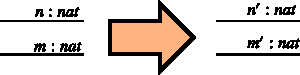
\includegraphics{diagrams/nat-nat1.pdf}
\end{center}

Now numbers can be implemented by the recursive type {{nat = @@x.1+x}}
in {{langRevT}}. This gives us the isomorphisms 

\begin{center}
  {{unfold : nat <-> 1 + nat : fold}}
\end{center}

We start by examining the first value. 

\begin{center}
  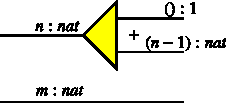
\includegraphics{diagrams/nat-nat2.pdf}
\end{center}

\item
The triangle denotes the {{unfold}} isomorphism, which works as
follows: If the number {{n}} is zero, the output is the top branch
which has type {{1}}. If the number was non-zero, the output is on the
bottom branch and has value {{n-1}}. 

Since the abstract machine increments second component, we know that
we need a {{fold}} on the second component to accomplish this. So we
can fill in the output part of the interpreter dually. 

\begin{center}
  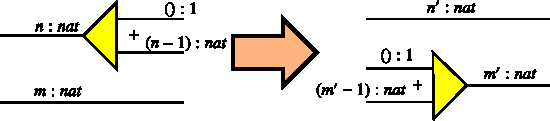
\includegraphics{diagrams/nat-nat3.pdf}
\end{center}

\item
Let us examine all the possible input states, by distributing on the
input. Dually let us do the same with the output, but this time also
be a little bit explicit about the swap operations required so the
right types are in place.

\begin{center}
  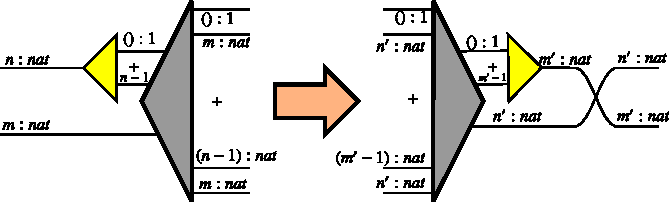
\includegraphics{diagrams/nat-nat4.pdf}
\end{center}

\item
The construction above already gives us some insight into how we can
implement our one reduction step. If we chose {{m = m'-1}} and we
chose {{n-1 =n'}} then we have essentially encoded the required
rewrite. Lets state this in words - the new value of {{n}}, namely
{{n'}}, is equal to {{n-1}}. And further - the new value of {{m}},
namely {{m'}}, is {{m+1}} (because {{m'-1=m}}). 

We can thus connect the lower branches with the appropriate
isomorphism to reflect this relationship. In this case the isomorphism
is just a swap of the two wires involved.

\begin{center}
  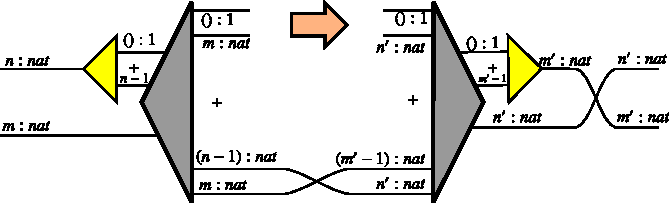
\includegraphics{diagrams/nat-nat5.pdf}
\end{center}

\item
We are a few steps away from an interpreter at this point and the
final steps rely on the answers to a few questions.

\begin{enumerate}
\item How do relate the outputs of the combinator to the inputs, such
  that the machine correctly takes multiple steps?

\item What do we do about the two inner branches? 

\end{enumerate}

The branch labeled {{((), m)}} looks like the stop state of the
machine. The branch label-led {{((), n')}} looks like the start state
of the program. To complete the interpreter, we flip our current
construction inside out.

\begin{center}
  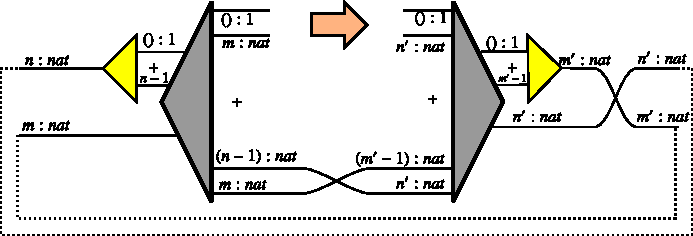
\includegraphics{diagrams/nat-nat6.pdf}
\end{center}

Which gives us

\begin{center}
  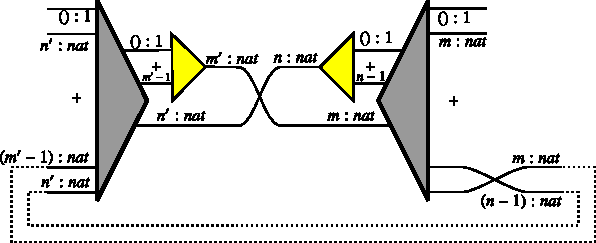
\includegraphics{diagrams/nat-nat7.pdf}
\end{center}

This basically completely our construction of the interpreter. We
basically need to use a {{trace}} to feedback related machine states
to related machine states.

\begin{center}
  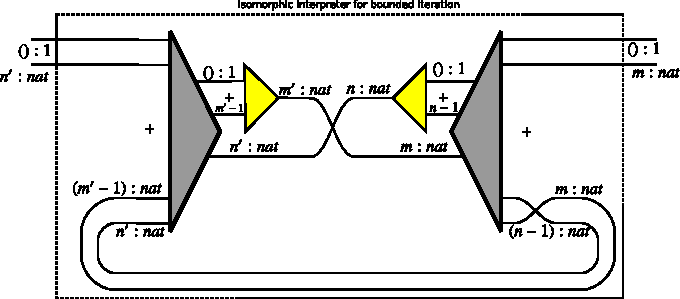
\includegraphics{diagrams/nat-nat8.pdf}
\end{center}

\end{enumerate}

%%%%%%%%%%%%%%%%%%%%%%%%%%%%%%%%%%%%%%%%%%%%%%%%%%%%%%%%%%%%%%%%%%%%%%%%%%%%%%%%%%%%%
\section{Abstracting out the Construction}

%%%%%%%%%%%%%%%%%%%%%%%%%%%%%%%%%%%%%%%%%%%%%%%%%%%%%%%%%%%%%%%%%%%%%%%%%%%%%%%%%%%%%
\subsection{What are the high level steps in the translation?}
\label{sec:steps}

TODO

\begin{enumerate}
\item Expand the input such that every input term that the LHS of the
  interpreter pattern matches on is exposed.

\item Expand the output such that every output term that it
  reconstructed by the interpreter is exposed.

\item Shuffle matching LHS term to matching RHS terms, inserting any
  appropriate mediating computations. In the previous example, this
  was only a swap operation.

\end{enumerate}

%%%%%%%%%%%%%%%%%%%%%%%%%%%%%%%%%%%%%%%%%%%%%%%%%%%%%%%%%%%%%%%%%%%%%%%%%%%%%%%%%%%%%
\subsection{What abstract machines can be turned into isomorphic interpreters?}

Logically reversible abstract machines with distinguishable start and
stop states can be converted into isomorphic interpreters in
{{langRevT}}.  To develop an understanding for what sorts of machines
these are, let us look at some examples.

Consider a machine with the following two reduction steps
 and . Can we create an
isomorphic interpreter for such a machine? We can't, because for any
given machine state, it is not obvious what reduction rule to
apply. We could reverse this machine if there was a clear
non-ambiguity in which machine rule was chosen.

Consider a machine, with the following rewrite rules
 and . Can we
create an isomorphic interpreter for this machine? It turns out we
can't because for any given output state  it is not
obvious which input state it came from - i.e. there are two
possibilities  or there is .

Consider a machine that has the addition rule 
where {{z}} is the sum of {{x}} and {{y}}. This machine again cannot
be turned into an isomorphic interpreter because the one reduction
rule does not have a logically inverse -- in other words, given a
{{z}}, we are unable to determine which {{x}} and {{y}} it originated
from.

If we had only the reduction relation , can we
construct an isomorphic interpreter? After all, every rewrite rule is
logically reversible. In fact, this is not possible because there is
no distinguished start state for such an interpreter and hence one
does not know when to stop during reverse execution.

\noindent
Conditions that must be satisfied for constructing a isomorphic
interpreter:

\begin{enumerate}

\item Distinguishable start and stop states. There may be more than one
  valid start state and more than one valid stop state.

\item Each valid machine state must match a unique reduction LHS. Each
  valid machine state must machine a unique reduction RHS.

\item Every reduction step must be computable (in {{langRevT}}) and
  must be logically reversible -- i.e. it must be possible to reduce
  from right to left.

\end{enumerate}


%%%%%%%%%%%%%%%%%%%%%%%%%%%%%%%%%%%%%%%%%%%%%%%%%%%%%%%%%%%%%%%%%%%%%%%%%%%%%%%%%%%%%
\section{Adder and Multiplier}

\subsection{Logically Reversible Adder}

%subcode{bnf} include main
% Expressions, e = n
% Numbers, n, m,p = 0 | n + 1
%
% Machine states = <e, e, e>
% Start state = <n, p, 0>
% Stop State = <0, p', m>

Small-step Operational semantics:

%subcode{opsem} include main
% <n+1, p, m> |--> <n, p+1, m+1>

This is an ostensibly useful machine in the sense that it computes the
sum of its two inputs.  This construction proceeds exactly like the
previous one till we have the following situation:

\begin{center}
  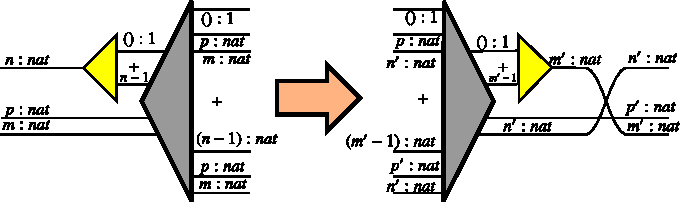
\includegraphics{diagrams/adder1.pdf}
\end{center}

The equalities we would like to express at this point are {{n-1=n'}},
{{m=m'-1}} and that {{p+1=p'}}. Fortunately {{langRevT}} provides the
{{add1: nat <-> nat}} combinator and so we could just use that to
mediate between {{p}} and {{p'}}. This is one solution and this gives
us:

\begin{center}
  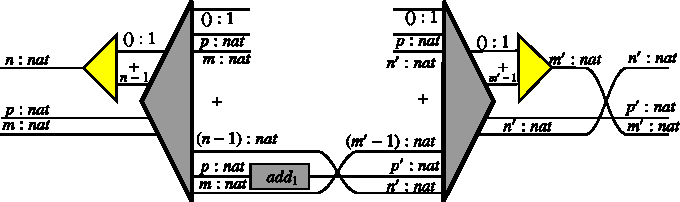
\includegraphics{diagrams/adder2.pdf}
\end{center}

This can be inverted as before, to give us an interpreter. While this
is a correct implementation of the small-step semantics, it is
somewhat unsatisyfing for the reason that it does not see very
systematic. After all we chose to use an {{add1}} for {{p}} -- why
didn't we do the same for {{m}}? More importantly, the fact that we
chose used {{add1}} is also hiding something -- namely that {{add1}}
is a partial isomorphism. Its inverse is not defined when applied to
{{0}} i.e. it will go into an infinite loop. 

In a sense this implicit assymetry of the abstract machine was being
hidden by the {{add1}} operation. So instead of chosing to use
{{add1}} let us chose to expand out {{p'}}, as recommended by step 2
in section \ref{sec:steps}. This gives us the following: 


\begin{center}
\scalebox{0.9}{
  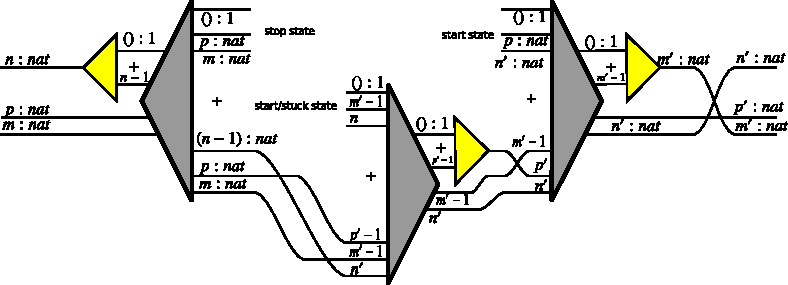
\includegraphics{diagrams/adder3.pdf}
}
\end{center}






%%%%%%%%%%%%%%%%%%%%%%%%%%%%%%%%%%%%%%%%%%%%%%%%%%%%%%%%%%%%%%%%%%%%%%%%%%%%%%%%%%%%%
\section{Tree Traversal}

%%%%%%%%%%%%%%%%%%%%%%%%%%%%%%%%%%%%%%%%%%%%%%%%%%%%%%%%%%%%%%%%%%%%%%%%%%%%%%%%%%%%%
\section{A {{langRev}} Interpreter}





\bibliographystyle{splncs03} 
\bibliography{cites}
\end{document}

